\documentclass[11pt, a4paper]{article}
% \documentclass{article}
\usepackage{tikz}
\usepackage{amsmath}
\usepackage[utf8]{inputenc}
\usepackage[hungarian]{babel}
\usetikzlibrary{calc}

\begin{document}
H\'uzzunk egy $e$ egyenest \'es az $e$ egynessel p\'arhuzamossan egy $f$ egyenest. Mivel az egyenesek p\'arhuzamossak, b\'armely pont az $e$ egyenesen, az $f$ egyenest\H{o}l egyenl\H{o} t\'avols\'agra van. Term\'eszetessen ez az \'all\'it\'as ford\'itva is igaz. Vagyis b\'armely pont az $f$ egyenesen, az $e$ egyenest\H{o}l egyenl\H{o} t\'avols\'agra van.

\begin{figure}[h]
\centering
\begin{tikzpicture}
  \node (e1) at (-3.5, 0.0) {$e$};
  \node (e2) at ( 3.5, 0.0) {};
  \node (f1) at (-3.5, 2.0) {$f$};
  \node (f2) at ( 3.5, 2.0) {};
  
  \node (A) at (-2.0, 0.0) [label=below:$A$] {};
  \node (B) at ( 1.0, 0.0) [label=below:$B$] {};
  \node (C) at ( 0.0, 2.0) [label=above:$C$] {};
  
  \draw (e1) -- (e2);
  \draw (f1) -- (f2);
  
  \filldraw (A) circle (1pt);
  \filldraw (B) circle (1pt);
  \filldraw (C) circle (1pt);
\end{tikzpicture}
\caption{P\'arhuzamos egyenesek}
\label{fig:paralel}
\end{figure}
P\'eldaul az \ref{fig:paralel} \'abr\'an egy $A$ \'es $B$ pontot l\'atunk az $e$ egyenesen \'es egy $C$ pontot az $f$ egyenesen. Az $A$ \'es a $B$ pont ugynakkora t\'avols\'agra van az $e$ egyenest\H{o}l, mint a $C$ pont az $f$ egyenest\H{o}l.

Ha az $A$ pontot össze kötjük a $C$ ponttal \'es ugyanezt tesszük a $B$ \'es $C$ ponttal, akkor egy h\'aromszöget kapunk.

\begin{figure}[h]
\centering
\begin{tikzpicture}
  \node (e1) at (-3.5, 0.0) {$e$};
  \node (e2) at ( 3.5, 0.0) {};
  \node (f1) at (-3.5, 2.0) {$f$};
  \node (f2) at ( 3.5, 2.0) {};
  
  \draw (-2.0, 0.0) -- (0.0, 2.0) -- (1.0, 0.0);

  \node (A) at (-2.0, 0.0) [label=below:$A$] {};
  \node (B) at ( 1.0, 0.0) [label=below:$B$] {};
  \node (C) at ( 0.0, 2.0) [label=above:$C$] {};

  \draw (e1) -- (e2);
  \draw (f1) -- (f2);
  
  \filldraw (A) circle (1pt);
  \filldraw (B) circle (1pt);
  \filldraw (C) circle (1pt);
\end{tikzpicture}
\caption{Egy h\'aromszög}
\label{fig:tri1}
\end{figure}

Mozgassuk el a $C$ pontot az $f$ egyenes ment\'en egy kevesset balra. Akkor a következ\H{o} k\'epet kapjuk meg. 

\begin{figure}[h]
\centering
\begin{tikzpicture}
  \node (e1) at (-3.5, 0.0) {$e$};
  \node (e2) at ( 3.5, 0.0) {};
  \node (f1) at (-3.5, 2.0) {$f$};
  \node (f2) at ( 3.5, 2.0) {};
  
  \draw (-2.0, 0.0) -- (-0.8, 2.0) -- (1.0, 0.0);

  \node (A) at (-2.0, 0.0) [label=below:$A$] {};
  \node (B) at ( 1.0, 0.0) [label=below:$B$] {};
  \node (C) at (-0.8, 2.0) [label=above:$C$] {};

  \draw (e1) -- (e2);
  \draw (f1) -- (f2);
  
  \filldraw (A) circle (1pt);
  \filldraw (B) circle (1pt);
  \filldraw (C) circle (1pt);
\end{tikzpicture}
\caption{Egy m\'asik h\'aromszög}
\label{fig:tri1}
\end{figure}

A k\'et h\'aromszög területe egyenl\H{o}. Ugyanis az $\overline{AB}$ szakasz mind k\'et esetben megegyezik \'es a magass\'aga a k\'et h\'aromszögnek nem v\'altozott.

Eml\'ekeztet\H{o} a h\'aromszög terület\'enek egyenlete ha a területet $T$-vel az $\overline{AB}$ szakaszt $a$-val \'es a h\'aromszög magass\'ag\'at $m$-mel jelöljük:
\[
    T=\frac{a\cdot m}{2}
\]

A terület k\'eplete levezethet\H{o} k\'et der\'ekszög\H{u} h\'aromszög terület\'eb\H{o}l. Teh\'at ha a der\'ekszög\H{u} h\'aromszög terület\'et le tudjuk vezetni, akkor egy \'altal\'anos h\'aromszög terület\'et is ki tudjuk sz\'amolni. Toljuk el a $C$ ponot addig, hogy az $A$ ponttal összekötött egyenes egy der\'ekszöget k\'epezzen az $e$ egyenessel (ez az egyenes der\'ekszöget k\'epez az $f$ egyenessel is).

\begin{figure}[h]
\centering
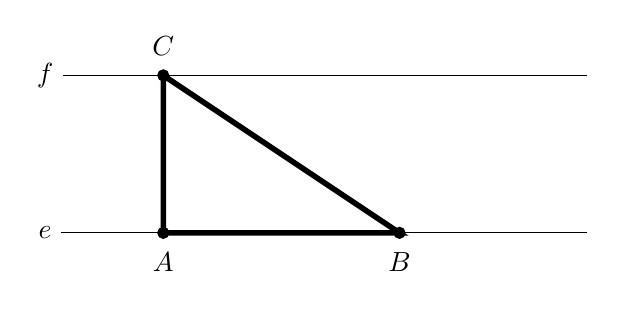
\begin{tikzpicture}
  \node (e1) at (-3.5, 0.0) {$e$};
  \node (e2) at ( 3.5, 0.0) {};
  \node (f1) at (-3.5, 2.0) {$f$};
  \node (f2) at ( 3.5, 2.0) {};
  
  \draw[line width=2pt] (-2.0, 0.0) -- (-2.0, 2.0) -- (1.0, 0.0) -- (-2.0, 0.0);

  \node (A) at (-2.0, 0.0) [label=below:$A$] {};
  \node (B) at ( 1.0, 0.0) [label=below:$B$] {};
  \node (C) at (-2.0, 2.0) [label=above:$C$] {};

  \draw (e1) -- (e2);
  \draw (f1) -- (f2);
  
  \filldraw (A) circle (2pt);
  \filldraw (B) circle (2pt);
  \filldraw (C) circle (2pt);
\end{tikzpicture}
\caption{Der\'ekszög\H{u} h\'aromszög}
\label{fig:tri1}
\end{figure}

Szerkessünk az $e$ egyenesre mer\H{o}leges egyenest a $B$ ponton keresztül. Ez az egyenes az $f$ egyenest egy $D$ pontban fogja metzeni. Az egyenesek, amellyek az $ABCD$ pontokat összekötik egy t\'eglalapot k\'epeznek.

\begin{figure}[h]
\centering
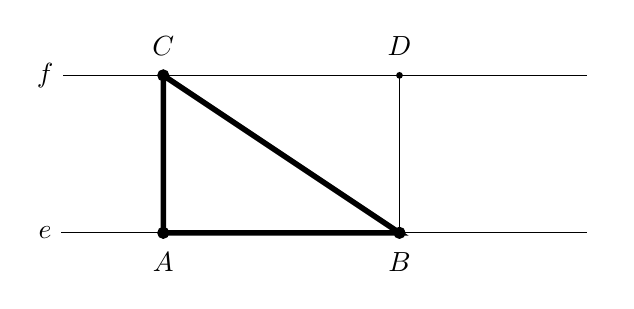
\begin{tikzpicture}
  \node (e1) at (-3.5, 0.0) {$e$};
  \node (e2) at ( 3.5, 0.0) {};
  \node (f1) at (-3.5, 2.0) {$f$};
  \node (f2) at ( 3.5, 2.0) {};
  
  \draw [line width=2pt] (-2.0, 0.0) -- (-2.0, 2.0) -- (1.0, 0.0) -- (-2.0, 0.0);
  \draw (1.0, 0.0) -- ( 1.0, 2.0);

  \node (A) at (-2.0, 0.0) [label=below:$A$] {};
  \node (B) at ( 1.0, 0.0) [label=below:$B$] {};
  \node (C) at (-2.0, 2.0) [label=above:$C$] {};
  \node (D) at ( 1.0, 2.0) [label=above:$D$] {};

  \draw (e1) -- (e2);
  \draw (f1) -- (f2);
  
  \filldraw (A) circle (2pt);
  \filldraw (B) circle (2pt);
  \filldraw (C) circle (2pt);
  \filldraw (D) circle (1pt);
\end{tikzpicture}
\caption{Der\'ekszög\H{u} h\'aromszög}
\label{fig:tri1}
\end{figure}

A t\'eglalap területe definici\'o szerint
\[T := a\cdot b\]
ha az $\overline{AB}$ szakaszt $a$-val \'es az $\overline{AC}$ szakaszt $b$-vel jelöljük. Teh\'at szavakban: A t\'eglalap területe egyenl\H{o} alap szor magass\'ag. Az $ABCD$ t\'eglalapot az $\overline{CB}$ szakasz megfelezi. Ebb\H{o}l következik a $ABC$ h\'aromszög területe a t\'eglalap terület\'enek fele.
\newpage
T\'erjünk vissza az \'altal\'anos h\'aromszöghöz. Itt k\'et esetet kell megvizsg\'alni. Az els\H{o} esethez tekintsük meg a következ\H{o} k\'epet.

\begin{figure}[h]
\centering
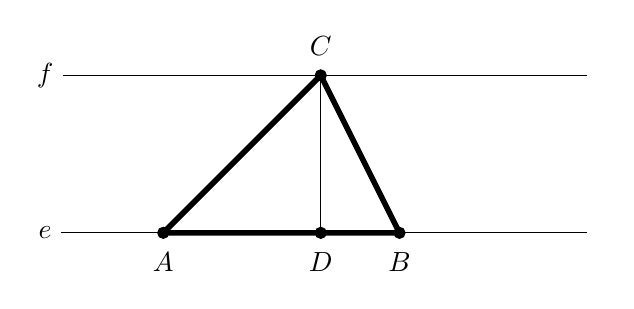
\begin{tikzpicture}
  \node (e1) at (-3.5, 0.0) {$e$};
  \node (e2) at ( 3.5, 0.0) {};
  \node (f1) at (-3.5, 2.0) {$f$};
  \node (f2) at ( 3.5, 2.0) {};
  
  \draw [line width=2pt] (-2.0, 0.0) -- (0.0, 2.0) -- (1.0, 0.0) -- (-2.0, 0.0);
  \draw (0.0, 2.0) -- (0.0, 0.0);

  \node (A) at (-2.0, 0.0) [label=below:$A$] {};
  \node (B) at ( 1.0, 0.0) [label=below:$B$] {};
  \node (C) at ( 0.0, 2.0) [label=above:$C$] {};
  \node (D) at ( 0.0, 0.0) [label=below:$D$] {};

  \draw (e1) -- (e2);
  \draw (f1) -- (f2);
  
  \filldraw (A) circle (2pt);
  \filldraw (B) circle (2pt);
  \filldraw (C) circle (2pt);
  \filldraw (D) circle (2pt);
\end{tikzpicture}
    \caption{Az els\H{o} eset}
\label{fig:tri1}
\end{figure}

Itt a $C$ pontb\'ol az $f$ egyenesre mer\H{o}legessen egy egyenest h\'uztunk. Ez az egyenes az $e$ egyenest a $D$ pontban metszi. A $\overline{CD}$ szakasz a $ABC$ h\'aromszöget k\'et r\'eszre v\'agja sz\'et. \'Igy a $ABC$ h\'aromszögb\H{o}l egy $ADC$ \'es egy $BDC$ h\'aromszög adodik. Ez \'altal a $ABC$ h\'aromszög területe megegyezik a k\'et kisebb h\'aromszög terület\'enak összeg\'evel. Egy k\'eplet levezet\'ese \'erdek\'eben jelöljük az $\overline{AD}$ szakasz hossz\'at $a_1$-gyel \'es a $\overline{DB}$ szakasz\'et $a_2$-vel. Ebb\H{o}l adodik az $\overline{AC}$ szakasz hossza, jelöljük $a$-val, megegyezik az $\overline{AD}$ \'es az $\overline{DB}$ szakaszok hossz\'anak összeg\'evel. Tehat
\[
a = a_1 + a_2
\]
Jelöljük az $ADC$ h\'aromszög terület\'et $T_1$-gyel \'es a $BDC$ h\'aromszög terület\'et $T_2$-vel. Akkor

\begin{align}
 \begin{aligned}
     T_1 &= \frac{a_1\cdot b}{2} \\
     T_2 &= \frac{a_2\cdot b}{2}
 \end{aligned}
 \end{align}

 Ha az elmondottak szerint az $ABC$ h\'aromszög terület\'et $T$-vel jelöljük akkor
 \[
  T = T_1 + T_2
 \]
Behejetes\'itjük a $T_1$-gyet \'es a $T_2$-t\H{o}t a fenti egyenlet jobb oldal\'aba, akkor
 \[
     T = \frac{a_1\cdot b}{2} + \frac{a_2\cdot b}{2} = \frac{a_1\cdot b + a_2\cdot b}{2} = \frac{(a_1 + a_2) \cdot b}{2} = \frac{a\cdot b}{2}
 \]

Ez \'altal el\'ertük az els\H{o} eset v\'eg\'et \'es megkaptuk a h\'aromszög terület\'enek kisz\'am\'it\'as\'ahoz \'erv\'enyes formul\'at.
\newpage
A m\'asodik esethez is tekintsük meg egy \'abr\'at.

\begin{figure}[h]
\centering
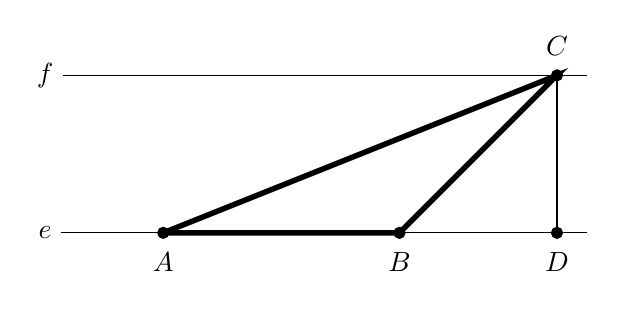
\begin{tikzpicture}
  \node (e1) at (-3.5, 0.0) {$e$};
  \node (e2) at ( 3.5, 0.0) {};
  \node (f1) at (-3.5, 2.0) {$f$};
  \node (f2) at ( 3.5, 2.0) {};
  
  \draw [line width=2pt] (-2.0, 0.0) -- (3.0, 2.0) -- (1.0, 0.0) -- (-2.0, 0.0);
  \draw (3.0, 2.0) -- (3.0, 0.0);

  \node (A) at (-2.0, 0.0) [label=below:$A$] {};
  \node (B) at ( 1.0, 0.0) [label=below:$B$] {};
  \node (C) at ( 3.0, 2.0) [label=above:$C$] {};
  \node (D) at ( 3.0, 0.0) [label=below:$D$] {};

  \draw (e1) -- (e2);
  \draw (f1) -- (f2);
  
  \filldraw (A) circle (2pt);
  \filldraw (B) circle (2pt);
  \filldraw (C) circle (2pt);
  \filldraw (D) circle (2pt);
\end{tikzpicture}
    \caption{A m\'asodik eset}
\label{fig:tri1}
\end{figure}

Itt ism\'et k\'et h\'aromszög seg\'its\'eg\'evel lehet erl\'erni a c\'elunkat. Az els\H{o} h\'aromszög az $ADC$ \'es a m\'asodik pedig az $BDC$ lesz. A különbs\'eg az els\H{o} esethez az, hogy itt a kereset h\'aromszög területe k\'et h\'aromszög különbs\'eg\'eböl sz\'am\'ithat\'o ki. Teh\'at az $ADC$ h\'aromszögb\H{o}l kiv\'agjuk a $BDC$ h\'aromszöget. Ehhez vegyük \'eszre, hogy a $\overline{AB}$ szakasz hossza, a $\overline{AD}$ szakasz hossz\'ab\'ol lev\'agott $\overline{BD}$ szakasz hossz\'aval egyenl\H{o}. Ha most az $\overline{AB}$ szakasz hossz\'at $a$-val jelöljük, tov\'abb\'a a $\overline{AD}$ szakasz hossz\'at $a_1$-gyel \'es a $\overline{BD}$ szakasz hossz\'at $a_2$-vel jelöljük, akkor

\[
 a = a_1 - a_2
\]

Mondottak szerint a keresett h\'aromszög területe
\[
 T = T_1 - T_2
\]
ha az $ADC$ h\'aromszög terület\'et $T_1$-gyel \'es a $BDC$ h\'aromszög terület\'et $T_2$-vel \'irjuk le. Mivel a $T_1$-gyel \'es a $T_2$-vel jelölt h\'aromszögek der\'ekszög\H{u} h\'aromszögek
\begin{align}
 \begin{aligned}
     T_1 &= \frac{a_1\cdot b}{2} \\
     T_2 &= \frac{a_2\cdot b}{2}
 \end{aligned}
 \end{align}

Ism\'et behejetes\'itjük a $T_1$-gyet \'es a $T_2$-t\H{o}t a fenti egyenlet jobb oldal\'aba, akkor
 \[
     T = \frac{a_1\cdot b}{2} - \frac{a_2\cdot b}{2} = \frac{a_1\cdot b - a_2\cdot b}{2} = \frac{(a_1 - a_2) \cdot b}{2} = \frac{a\cdot b}{2}
 \]
\newpage
Egy harmadik esetet is elk\'epzelhetünk. De ha j\'ol \'atgondoljuk ezt az esetet, akkro es az eset a m\'asodit eset tükörk\'epe.

\begin{figure}[h]
\centering
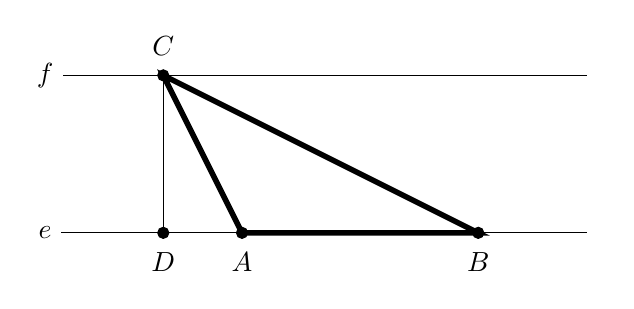
\begin{tikzpicture}
  \node (e1) at (-3.5, 0.0) {$e$};
  \node (e2) at ( 3.5, 0.0) {};
  \node (f1) at (-3.5, 2.0) {$f$};
  \node (f2) at ( 3.5, 2.0) {};
  
  \draw [line width=2pt] (-1.0, 0.0) -- (-2.0, 2.0) -- (2.0, 0.0) -- (-1.0, 0.0);
  \draw (-2.0, 2.0) -- (-2.0, 0.0);

  \node (A) at (-1.0, 0.0) [label=below:$A$] {};
  \node (B) at ( 2.0, 0.0) [label=below:$B$] {};
  \node (C) at (-2.0, 2.0) [label=above:$C$] {};
  \node (D) at (-2.0, 0.0) [label=below:$D$] {};

  \draw (e1) -- (e2);
  \draw (f1) -- (f2);
  
  \filldraw (A) circle (2pt);
  \filldraw (B) circle (2pt);
  \filldraw (C) circle (2pt);
  \filldraw (D) circle (2pt);
\end{tikzpicture}
    \caption{A m\'asodik eset}
\label{fig:tri1}
\end{figure}

Teh\'at az argument\'aci\'o ugyanaz lesz mint a m\'asodik esetben.


\end{document}

